% Created:  Thu 10 Jul 2014 04:22 PM
% Author:   Josh Wainwright
% Filename: quadtree-traversal.tex

\section{Quadtree Traversal}
\label{sec:quadtree_traversal}

Whether the quadtree is stored in memory as a recursive quadtree data
structure, or as hash table, Section~\ref{sub:hash_table_implementation}, the
most important and computationally intensive step is extracting the clusters at
the correct depth and disregarding those data points that can be attributed to
noise.

The quadtree numbering system chosen lends itself very well to analysis based
on spatial location and the proximity of neighbours to a given node being
examined.

\subsection{Algorithm Description}
\label{sub:algorithm_description}

To \emph{propagate} is defined as the act of ``spreading and promoting (an
idea, theory etc.) widely''\cite{oed31}. This term shall refer to the process
by which a single starting location, previously chosen, is expanded by
examining neighbours to form a cluster. The algorithm is defined recursively
with the main step being `propagation' of nodes. The propagation algorithm is
performed as follows:

\begin{enumerate}
	\item Choose a starting location that has not yet been checked, $l$.
	\item For this given starting location, the $i$ neighbours surrounding it,
		$n_0$ to $n_i$, are checked for validity based on the conditions of the
		analysis (the way these neighbours are selected is discussed in
		Section~\ref{sub:choosing_neighbours}).
	\item If a node fails the check, then it is recorded as having done so and
		shall not be checked again. If it passes, then it is, itself,
		propagated.
		\begin{itemize}
			\item To be ``propagated'' means to perform this propagation
				algorithm using that node as the starting location.
		\end{itemize}
	\item When all nodes have been checked, return to step 1.
	\item The algorithm completes either when;
	\begin{itemize}
		\item every one of the nodes in the image have been checked and
			included or ignored, or
		\item the cluster has ended, so all the neighbours of all checked nodes
			have failed the validity tests and no further starting locations
			were found or specified.
	\end{itemize}
\end{enumerate}

This process is shown graphically in Figure~\ref{fig:propogation}.

\begin{figure}[tbh]
	\centering
	\includegraphics[width=7cm]{propogation.pdf}

	\caption[Propagation of a cluster from a starting location.]{For a starting
		location, (a), in an image, no information is known and so all its
		neighbours are checked. Some of these are found to be part of the
		cluster, others are rejected. The ones that are included are then,
		themselves, checked and so on. As the cluster grows, (b), (c) and
		(d), the number of checked nodes increases.}\label{fig:propogation}
\end{figure}

Listing~\ref{code:quadtree-propagate} shows pseudo code for the propagate
algorithm which, starting at a given starting location, expands the cluster
outwards while there still exist valid neighbours that should be included. The
\texttt{getNeighbours()} method is described in
Section~\ref{sub:choosing_neighbours}. This is a recursively defined algorithm
which calls itself for each of the neighbours of a node and for each of their
neighbours, and so on. There is a condition that prevents the algorithm from
being called again on nodes that have been checked already. This prevents a
loop from forming and preventing the algorithm terminating.

\begin{center}
\begin{minipage}{\textwidth}
\begin{lstlisting}[caption={[Code for the propagate algorithm.]Code for the
	propagate algorithm which expands an initial starting location to a
	cluster.}, label=code:quadtree-propagate]
	function |propagate()| {
		node[] startLocations = getStartLocations() (*@\label{eql:a}@*)
		for each node in startLocations
			propagate(node)
	}

	function |propagate(node)| {
		if (not node.inCluster()) (*@\label{eql:b}@*)
			node[] neighbours = getNeighbours(node)

			for each n in neighbours  (*@\label{eql:c}@*)
				if (n is valid) propagate(n)
	}
\end{lstlisting}
\end{minipage}
\end{center}

In reference to Listing~\ref{code:quadtree-propagate} above:
\begin{description}
	\item[Line~\ref{eql:a}] A set of starting locations is selected based on
		some heuristic that determines if a node is deep enough in the tree to
		be used as a starting location.

	\item[Line~\ref{eql:b}] Nodes are only propagated if they have not already
		been included in a cluster. If this were not the case, then clusters
		would overlap.

	\item[Line~\ref{eql:c}] Each of the neighbours of the current node is
		propagated. The method of choosing neighbours determines how far the
		cluster can spread, and is separated from the clustering algorithm.
\end{description}

When discovering clusters via this propagation technique, care must be taken to
avoid a run-away situation where every node in the tree gets included. This
would happen when looking at the neighbours of a node and blindly including
them. Since every internal node has exactly four neighbours, the propagation
would terminate only when reaching the boundary nodes. Instead, the depth of
the node must be considered. Again, the simplest method is not sufficient. If
the propagation is limited to a given node depth, even if this is not the same
as the deepest node, the size of any clusters that are identified will be
limited, as shown in Figure~\ref{fig:propogation-halting}.  Since the depth to
consider is not able to change, when the neighbours of the blue node are
checked, no correct neighbours are found and so the process terminates. When
able to view the larger structure of the nodes, however, it is clear that the
structure continues beyond the gap, following the dotted line.

\begin{figure}[tbh]
	\centering
	\begin{subfigure}[c]{5.2cm}
		\includegraphics[width=\linewidth]{propogation-halting.pdf}
		\caption{}\label{fig:propogation-halting}
	\end{subfigure}%
	\quad
	\begin{subfigure}[c]{3.2cm}
		\includegraphics[width=\linewidth]{propogation-levels.pdf}
		\caption{}\label{fig:propogation-levels}
	\end{subfigure}

	\caption[Considerations regarding quadtree levels to be accepted.]
		{Considerations regarding quadtree levels that will be accepted
		when propagating a node in a quadtree. \subref{fig:propogation-halting}
		If the depth range that specifies how far up the tree to look for valid
		neighbours is too small then a cluster might be terminated too soon.
		\subref{fig:propogation-levels}(i) a depth range of two and, (ii) a
		depth range of three.}\label{fig:prop-levels-halting}
\end{figure}

To avoid this, a certain amount of leniency must be allowed when deciding what
constitutes a neighbour. Given an appropriate value, this would allow both of
the larger white cells in Figure~\ref{fig:propogation-halting} to be included.

The term \emph{depth range} shall define the levels that are to be considered
when choosing neighbours with respect to a target depth. Since clusters are
being considered as areas of increased density of points, all cells with a
depth greater than the target depth shall be allowed, so the purple cells in
Figure~\ref{fig:propogation-halting} would be included when the target depth is
the same as the depth of the included red cells. A depth range of zero is
equivalent to the situation above where only cells of a given depth are
considered. A depth range of one would mean that the white square in
Figure~\ref{fig:propogation-levels}\,(i) would be included but not in~(ii),
whereas a depth range of two would include both and so on.

\subsection{Clustering Start Locations}
\label{sub:clustering_start_locations}

In order for the algorithm to proceed correctly, a good initial node, a
starting location, must be chosen. Since the clusters to be found are regions
of high point density, it makes sense to start the clustering algorithm at the
point in the image with the highest point density. This should ensure that the
most defined cluster is always found with subsequent clusters being less dense,
and so less well defined.

When starting at the highest density node, i.e., the node which is at the
deepest level in the tree, propagating this node and then terminating; the
cluster shown in Figure~\ref{fig:single-cluster} is found. The file
\texttt{palm-1.txt} was used and generated this data in
\SI{457}{\milli\second}. This shows that the algorithm works correctly.
Altering the parameters that are used to generate the quadtree affects the size
of the nodes that are included in the cluster and the depth that is searched.

\begin{figure}[tbh]
	\centering
	\begin{subfigure}[c]{4.2cm}
		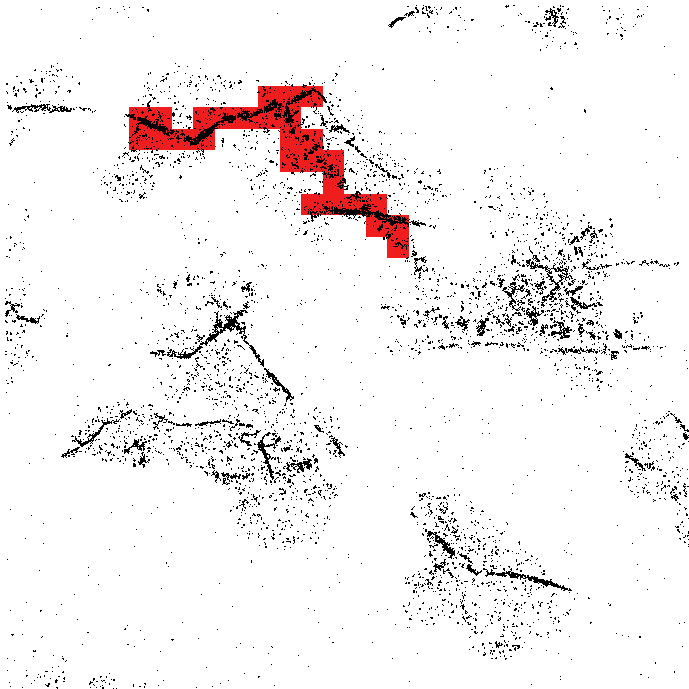
\includegraphics[width=\textwidth]{single-cluster.png}
		\caption{}\label{fig:single-cluster-points}
	\end{subfigure}%
	\quad
	\begin{subfigure}[c]{4.2cm}
		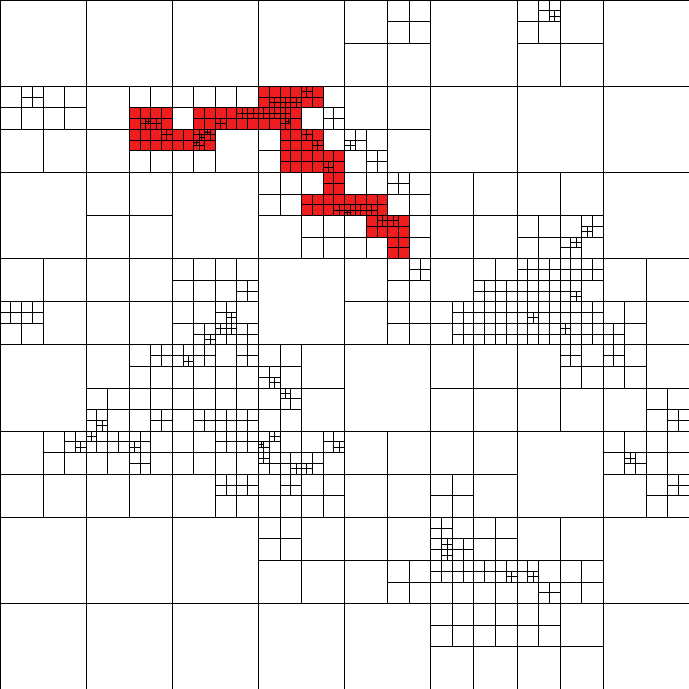
\includegraphics[width=\textwidth]{single-cluster-lines.png}
		\caption{}\label{fig:single-cluster-lines}
	\end{subfigure}

	\caption[Propagation of a single starting location.]{Initial versions of
		the clustering algorithm terminated immediately after finishing
		propagating the first cluster. This gives a useful test as to the
		correctness of the algorithm since there are no other clusters for this
		to collide with. It is useful to be able to check both
		\subref{fig:single-cluster-points} the points that were considered to
		be in the cluster and \subref{fig:single-cluster-lines} the nodes in
		the quadtree that were included and where the propagating algorithm
		stopped.}\label{fig:single-cluster}
\end{figure}

In order to find other clusters, the algorithm must be restarted with a new
starting location. This is chosen as the deepest node in the tree that is not
already included in a cluster. There are a number of different way to terminate
this process of finding new clusters:

\begin{itemize}

	\item Perform a set number of iterations. This performs well if the
		clusters to be located can be easily counted, but in the general case,
		this is not possible or desired. If the number of iterations is set to
		a high value, of the order of 50, the algorithm will continue to locate
		``clusters'' even if they do not exist and will eventually simply
		report the background noise as a cluster. To prevent this, a limit can
		be set on the depth a starting location must be in order to be valid.

	\item Continue iterating until a depth limit is reached. This is a more
		general form of the previous case, but for this case, the limit on the
		depth of a starting location will always be reached.

	\item Allow the user to make a number of starting point location selections
		manually. Since ImageJ allows multi-point region of interest (ROI)
		selections, the user could be asked to place a new ROI at the places
		they consider a reasonable place to find a cluster. The algorithm would
		then convert the locations of each of these ROI points into the
		relevant quadtree code and begin propagating from that node and
		terminate when all of the ROI's had been used. This suffers from the
		same issues as method 1, since it is not helpful to require the user to
		make the selections manually.

\end{itemize}

The plugin developed uses a combination of the first and second approaches.
Since the number of clusters cannot often be counted easily, the user cannot be
expected to provide this value. However, it is also very difficult to determine
when clusters that are being propagated are valid or not. The algorithm can be
instructed to halt if the nodes that are being considered are too high up the
tree, i.e., too many nodes have been included and the algorithm has run away,
but this is generally not sufficient for all cases. Instead, a comparison with
the depth range allowed (which is set by the user) with the difference between
the first cluster found and the current cluster is made. If the difference is
similar to the depth range, then the algorithm continues. After this process
has finished, the clusters that have been found are examined and those that are
too small with respect to the others are removed.

\begin{figure}[tbh]
	\centering
	\begin{minipage}[c]{7cm}
		\fbox{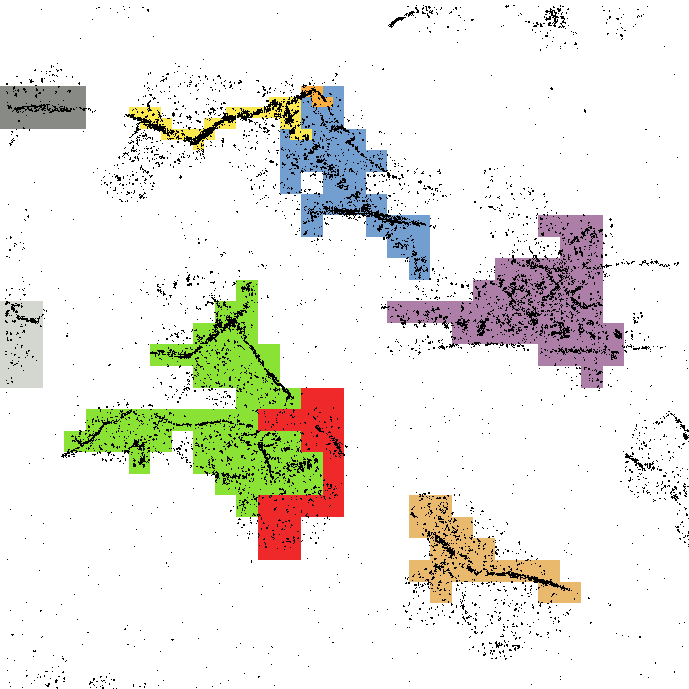
\includegraphics[width=\textwidth]{multiple-clusters-colours.png}}
	\end{minipage}%
	\,
	\begin{minipage}[c]{1cm}
		\centering
		\begin{tabular}[b]{l}
			\cellcolor{lyellow}1 \\
			\cellcolor{lorange}2 \\
			\cellcolor{lbrown}3 \\
			\cellcolor{lgreen}4 \\
			\cellcolor{lblue}5 \\
			\cellcolor{lpurple}6 \\
			\cellcolor{lred}7 \\
			\cellcolor{silver}8 \\
			\cellcolor{lgrey}9 \\
		\end{tabular}
	\end{minipage}

	\caption[Propagation of multiple starting locations.]{Initial versions of
		the clustering algorithm included too many nodes, making the clusters
		too large. This image shows how each node cluster that is started is
		independent of the previous ones. The clusters were identified in the
		order they are listed on the right.}\label{fig:multiple-clusters-colours}
\end{figure}

\subsection{Choosing Neighbours}
\label{sub:choosing_neighbours}

Some care must be taken when deciding what constitutes a neighbour of a node
and what does not. As mentioned above, when detecting clusters using
propagation, the neighbours of a node are checked and, if they are valid, are
themselves propagated. For this reason, a poor choice of neighbours means that
the propagation will either:

\begin{itemize}
	\item be cut short too early, and so not all of the clusters will be
		located, or
	\item include too many nodes, in which case the clusters will not represent
		the actual data.
\end{itemize}

The first neighbours that must be considered, named \emph{rook's case}
neighbours by~\citet{abel1990comparative}, are the four nodes that lie to the
north, east, south and west of the current node. These are the nodes that are
directly in contact with the node and so, if they are valid, represent a direct
continuation of the cluster.

However, if the choice of neighbours is limited to these four, some major
structures are missed. Figure~\ref{fig:kernel-rooks-case} shows how this
arrangement misses a large portion of the cluster, simply because the
propagation could not consider the nodes across the boundary. If, in addition
to the rook's case, the four \emph{diagonal} neighbours are included, giving a
total of eight, the results are much more complete, as shown in
Figure~\ref{fig:kernel-all8}.

\begin{figure}[tbh]
	\centering
	\begin{subfigure}[b]{4.2cm}
		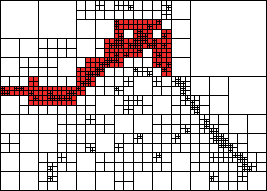
\includegraphics[width=\textwidth]{clusters/kernel-rooks-case.png}
		\caption{}\label{fig:kernel-rooks-case}
	\end{subfigure}%
	\quad
	\begin{subfigure}[b]{4.2cm}
		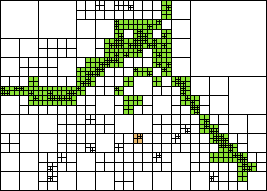
\includegraphics[width=\textwidth]{clusters/kernel-all8.png}
		\caption{}\label{fig:kernel-all8}
	\end{subfigure}

	\caption[A comparison of different neighbour sets.]{A comparison between
		different neighbour sets.  \subref{fig:kernel-rooks-case} shows how
		some of the cluster is lost when using just the rook's case neighbours,
		whereas, using all eight neighbours, Figure~\subref{fig:kernel-all8}
		more of the cluster is included.}\label{fig:kernel-options}
\end{figure}

\subsubsection{Image Kernel}
\label{ssub:Image Kernel}

The requirement to include eight neighbours for each node suggests that it
might be of value to allow users to specify an arbitrary number of neighbours
around the given cell.

In many applications in image processing, the concept of an image \emph{kernel}
is commonplace. This is a square, odd-sided matrix that is used to apply
filters and other effects to an image. The kernel is placed over each of the
pixels in the image in turn so that the central element in the matrix is over
the current pixel and each of the other elements is over another pixel. The
value of the element in the kernel is then used to manipulate the pixels in the
image below it. For example, to blur an image, a $3\times 3$ kernel composed of
all $\rfrac{1}{9}$'s can be used. When applied, this would mean that the
% TODO reread sentence
current pixel is given a value which is the sum of each of matrix elements
multiplied by the pixel value beneath it.

A similar technique is used here to choose neighbours from the quadtree. The
image kernel that is used is a binary matrix, meaning that all of the elements
are restricted to either 0 or 1, but, in all other respects, is the same as a
regular image kernel. The kernel is placed over a node of interest. Any node
that lies under an element with a value of 1 is included as a neighbour and
nodes under 0 elements are ignored. The value of the central element in the
kernel does not matter, but the convention is to set this to 1.

Thus, the simplest kernel, though of least use, is the identity kernel which
has an element with value `1' in the centre and all other elements `0',
Figure~\ref{fig:kernel-identity}. This would result in no neighbours being
selected, and so no clusters located. The rook's case neighbours are now
represented with the kernel in Figure~\ref{fig:kernel-image-rooks} and the case
with all 8 neighbours in Figure~\ref{fig:kernel-image-all8}.

\begin{figure}[tbh]
	\centering
	\begin{subtable}[b]{0.2\textwidth}
	\centering
		\begin{tabular}{|l|l|l|}
			\hline
			0 & 0 & 0 \\
			\hline
			0 & \cellcolor{lred}1 & 0 \\
			\hline
			0 & 0 & 0 \\
			\hline
		\end{tabular}
		\caption{}\label{fig:kernel-identity}
	\end{subtable}%
	\quad
	\begin{subtable}[b]{0.2\textwidth}
	\centering
		\begin{tabular}{|l|l|l|}
			\hline
			0 & 1 & 0 \\
			\hline
			1 & \cellcolor{lred}1 & 1 \\
			\hline
			0 & 1 & 0 \\
			\hline
		\end{tabular}
		\caption{}\label{fig:kernel-image-rooks}
	\end{subtable}%
	\quad
	\begin{subtable}[b]{0.2\textwidth}
	\centering
		\begin{tabular}{|l|l|l|}
			\hline
			1 & 1 & 1 \\
			\hline
			1 & \cellcolor{lred}1 & 1 \\
			\hline
			1 & 1 & 1 \\
			\hline
		\end{tabular}
		\caption{}\label{fig:kernel-image-all8}
	\end{subtable}

	\caption[Kernels for the identity matrix, rook's case and all 8
		neighbours.]{Kernels for~\subref{fig:kernel-identity} the identity
		matrix,\subref{fig:kernel-image-rooks} rook's case neighbours
		and~\subref{fig:kernel-all8} all 8 neighbours. The central cell of the
		kernel can be anything as it is never included as a neighbour.}\label{fig:kernel-neighbours}
\end{figure}

This functionality provides the ability to target certain types of clusters
depending on the spatial orientation of the cluster; vertical or horizontal
etc. Figure~\ref{fig:kernel-shapes} shows a number of possible kernel shapes
that would allow different types of clusters to be targeted. Each of these show
the central cell with the cells that would be represented by a 1; cells
represented by 0's are not displayed.

\begin{figure}[tbh]
	\centering
	\includegraphics[width=7cm]{kernel-shapes.pdf}

	\caption[Different kernel shapes for different clusters.]{Different kernel
		shapes can be used to find different sorts of clusters. (a)~The basic
		rook's case neighbours and (b)~the full number of closest neighbours
		are the simplest general cases, used for most clusters. (c)~The area to
		search can be extended by including more neighbours---this could help
		find clusters that are more sparsely populated. Clusters of a specific
		orientation can be located, for example, predominately (d)~vertical or
		(e)~NW SE diagonal.}\label{fig:kernel-shapes}
\end{figure}

\subsubsection{Searching Up and Down the Tree}
\label{ssub:searching_up_and_down_the_tree}

Once a node location has been identified as a valid neighbour, there is still
no guarantee that there exists a node there. There are three possible cases
concerning the location that has been identified. Each of these situations must
be handled differently in order to ensure that all of the correct nodes are
selected as neighbours.

\begin{enumerate}
	\item The location represents a leaf node, in which case the process is
		complete and a neighbour has been identified,
		Figure~\ref{fig:updownsearch}a.

		In this case, no further action must be taken.

	\item The location is to be a non-existent node, i.e., there may be a leaf
		node at a position further up the tree than the location meaning there
		is nothing at this position in the tree,
		Figure~\ref{fig:updownsearch}b.

		In this case, either the code that has been obtained from the kernel
		analysis must be shortened until it represents a node that exists in
		the tree, or the tree must be traversed according to the quadtree code
		until a leaf node is reached. The located node must then be compared
		against the node to which this is a neighbour to check that the two are
		within the depth range specified (Section~\ref{sub:option_sliders}).

	\item The location is a node in the quadtree which is not a leaf node,
		i.e., it has four children, each of which may be trees or leaves,
		Figure~\ref{fig:updownsearch}c.

		For this third case, the depth range is not considered since all nodes
		deeper than the starting node are assumed to be a part of the same
		cluster. Instead, all leaf nodes below the node represented by the code
		are included as valid neighbours, and hence are, themselves,
		propagated. To get these children, the sub-tree below the current node
		is traversed in pre- or post-order and every leaf node that is
		encountered is added as a neighbour.

\end{enumerate}

\begin{figure}[tbh]
	\centering
	\includegraphics[width=5cm]{updownsearch.pdf}
	\caption[Possible results of neighbour selection.]{The possible results of
		neighbour selection. The blue square is the node that is being
		propagated and the red square represents the location of the node given
		by the neighbour code, black squares are real nodes in the tree. (a)
		shows the ideal case where the neighbour is a node, (b) shows where the
		code could be further down in the tree than exists and (c) shows the
		case where a real node is selected, but is not a leaf.}\label{fig:updownsearch}
\end{figure}
